\documentclass[12pt]{article}
\usepackage[utf8]{inputenc}
\usepackage[english]{babel}

\usepackage{indentfirst}
\setlength{\parskip}{\baselineskip}
\usepackage{titling}
\renewcommand\thesection{\arabic{section}} 
\renewcommand\thesubsection{\thesection.\arabic{subsection}} 

\renewcommand{\footnotesize}{\fontsize{9pt}{11pt}\selectfont}

% \usepackage{fontspec}
%\setmainfont{Times New Roman}
\usepackage{hyphenat}
\usepackage{amsmath}
\usepackage{amssymb}
\setcounter{tocdepth}{3}
\usepackage{graphicx}
\graphicspath{{graphics/}}
\usepackage[export]{adjustbox}
\usepackage{algorithm}
\usepackage[noend]{algpseudocode}
\usepackage{url}
\usepackage{color}
\usepackage{multirow}
\usepackage{babel}

\usepackage[figurename=Exhibit]{caption}
\usepackage[tablename=Exhibit]{caption}
\usepackage[labelfont=bf]{caption}
\usepackage[shortlabels]{enumitem}
\usepackage{subcaption}
\usepackage{float}
\setcounter{secnumdepth}{3}

\usepackage{csquotes}
\usepackage[authordate,date=year,backend=biber,natbib]{biblatex-chicago}
% \usepackage{natbib}

\usepackage{apptools}
\usepackage{titlesec}
\titleformat{\section}{\bfseries}{\IfAppendix{\appendixname\ }{}\thesection.}{1em}{} 
\titleformat{\subsection}{\bfseries}{\hspace{2em}\thesubsection}{2em}{}
\titlespacing\section{0pt}{12pt plus 4pt minus 2pt}{0pt plus 2pt minus 2pt}
\titlespacing\subsection{-24pt}{12pt plus 4pt minus 2pt}{0pt plus 2pt minus 2pt}
\usepackage[title]{appendix}

\addbibresource{bibliography.bib}
\AtEveryBibitem{%
  \clearlist{language}%
}

\usepackage{standalone}
\usepackage{tikz}
\usepackage{xstring} 
\usepackage{url}


\usetikzlibrary{fit,positioning}
\usetikzlibrary{fadings}
\usetikzlibrary{decorations.pathreplacing}
\usetikzlibrary{shapes.geometric}


\newcommand{\specialcell}[2][c]{%
  \begin{tabular}[#1]{@{}c@{}}#2\end{tabular}}

\newcommand{\zp}[1]{{\textcolor{magenta} {#1}} }

\newcommand\drawNodes[2]{
  % #1 (str): namespace
  % #2 (list[list[str]]): list of labels to print in the node of each neuron
  \foreach \neurons [count=\lyrIdx] in #2 {
    \StrCount{\neurons}{,}[\arrlength] % uses the xstring package
    \foreach \n [count=\nIdx] in \neurons
      \node[neuron] (#1-\lyrIdx-\nIdx) at (2*\lyrIdx, \arrlength/2-1*\nIdx) {\n};
  }
}

\newcommand\denselyConnectNodes[2]{
  % #1 (str): namespace
  % #2 (list[int]): number of nodes in each layer
  \foreach \n [count=\lyrIdx, remember=\lyrIdx as \previdx, remember=\n as \prevn] in #2 {
    \foreach \y in {1,...,\n} {
      \ifnum \lyrIdx > 1
        \foreach \x in {1,...,\prevn}
          \draw[->] (#1-\previdx-\x) -- (#1-\lyrIdx-\y);
      \fi
    }
  }
}

\DeclareRobustCommand{\bbone}{\text{\usefont{U}{bbold}{m}{n}1}}
\DeclareMathOperator*{\argmax}{arg \ \!max}
\DeclareMathOperator{\EX}{\mathbb{E}}% expected value
\newcommand{\prior}{p(z)}
\newcommand{\posterior}{q_\phi(z|x)}
\newcommand{\likelihood}{p_\theta(x|z)}
\newcommand{\KL}{\mathrm{KL}\left(\posterior\,||\,\prior\right)}
\newcommand{\norm}[1]{\left\lVert#1\right\rVert}

\pagestyle{plain} 

\usepackage[left=1.0in,right=1.0in,top=1.0in,bottom=1.0in]{geometry}
\usepackage{fancyhdr} 
%\fancyhf{}
\cfoot{\thepage}
%\pagestyle{fancy} 
\usepackage{microtype}
\makeatletter 

\let\c@table\c@figure %
\let\ftype@table\ftype@figure %
\makeatother

\title{Variational Autoencoders:\linebreak  A Hands-Off Approach to Volatility}
\author{
\normalsize \textbf{Maxime Bergeron, Nicholas Fung, John Hull, Zissis Poulos\thanks {We would like to thank Ryan Ferguson, Vlad Lucic, Ivan Sergienko, Andreas Veneris and  Gary Wong  for their interest in this work as well as their many helpful comments. We would also like to thank Mitacs for providing financial support for this research.}}
}
\date{\today}

\begin{document}
% \sloppy
\tolerance=280
% \tolerance 200%/

\maketitle

{\parskip=0pt


  \noindent\textbf{Maxime Bergeron} is the Director of Research and Development at Riskfuel Analytics in Toronto, ON, Canada.

  \noindent\underline{mb@riskfuel.com}
  %\noindent <Address> %105 St George St, Toronto, ON M5S 3E6

  \vspace{0.5cm}
  \noindent\textbf{Nicholas Fung} is a Masters student in the Edward S. Rogers Sr. Department of Electrical \& Computer Engineering at the University of Toronto, and a Research Associate at Riskfuel Analytics in Toronto, ON, Canada.

  \noindent\underline{nfung@ece.utoronto.ca}
  \vspace{0.5cm}
 
    \noindent\textbf{John Hull} is a professor at the Joseph L. Rotman School of Management, University of Toronto.
    
    \noindent\underline{john.hull@rotman.utoronto.ca}
    
   %\noindent 105 St George St, Toronto, ON M5S 3E6
  
  \vspace{0.5cm}
  \noindent\textbf{Zissis Poulos} is a postdoctoral fellow at the Joseph L. Rotman School of Management, University of Toronto

\noindent\underline{zissis.poulos@rotman.utoronto.ca}

  %\noindent <Address>>%105 St George St, Toronto, ON M5S 3E6

\vspace{0.7cm}  
  \noindent Corresponding author:

\noindent\textbf{Nicholas Fung}

\noindent\underline{nfung@ece.utoronto.ca}
}

\newpage

\centerline{\bf\large Variational Autoencoders: A Hands-Off Approach to Volatility}

\begin{center}
  {Abstract}
\end{center}
% This article introduces a deep learning approach to modelling implied volatility surfaces in options markets. While traditional volatility models attempt to understand the underlying dynamics of the market, they sometimes fail to provide good predictions for anomalous data. We describe how an autoencoder can be trained to fit volatility surfaces in an entirely data-driven approach, and show that our model can provide good fits without making assumptions about markets. We show that by shifting the computational time upfront, our model can calibrate efficiently without sacrificing accuracy. We demonstrate how the learned model parameters can be explored, and how the model can be leveraged to construct realistic volatility surfaces using these parameters. Finally, we illustrate an example of our methodology by modelling an autoencoder on implied volatility surfaces observed in foreign exchange markets.

A volatility surface is an important tool for pricing and hedging derivatives. The surface shows the volatility that is implied by the market price of an option on an asset as a function of the option's strike price and maturity. Often, market data is incomplete and it is necessary to estimate missing points on partially observed surfaces. In this paper, we show how variational autoencoders can be used for this task. The first step is to derive latent variables that can be used to construct synthetic volatility surfaces that  are indistinguishable from those observed historically. The second step is to determine the synthetic surface generated by our latent variables that fits available data as closely as possible. As a dividend of our first step, the synthetic surfaces produced can also be used in stress testing, in market simulators for developing quantitative investment strategies,  and for the valuation of exotic options. We illustrate our procedure and demonstrate its power using foreign exchange market data.  


%Volatility surfaces are a fundamental tool used by theoreticians and practitioners alike to understand and participate in financial markets.  Since market data is often incomplete, there is a need to fill in missing points on partially observed surfaces.  This ishttps://www.overleaf.com/project/5fbc39b20b456d85c5f18038 traditionally done using  parametrizations rooted in various assumptions about the underlying dynamics of the market which often fail to provide good fits for anomalous data. 

%In this paper, we show that variational autoencoders (a specialized neural network architecture) can be used to produce practical volatility parametrizations with good fits in an entirely data driven manner without making such assumptions. In fact, they produce a moduli space of such parametrizations which allows us in turn to construct synthetic-yet-realistic volatility surfaces via sampling. To demonstrate our method concretely, we use one of the oldest and far-reaching sources of financial data: the foreign exchange market. Finally, we highlight that computational time is spent upfront during training, allowing for fast inference without compromising accuracy.

%To illustrate our approach concretely, we use one of the oldest and far-reaching sources of financial data: the foreign exchange market. We describe how our autoencoder architectures are chosen, how they are trained and how the resulting model's parameters can be interpreted. We then describe how the models can be leveraged to construct synthetic yet realistic volatility surfaces using these parameters. Finally, we highlight that as a byproduct of our approach (common to all deep learning techniques), computational time is spent upfront during training allowing for fast inference without compromising accuracy.
\vspace{0.5cm}


THREE KEY TAKEAWAYS:

\begin{enumerate}
  \item We show how synthetic yet realistic volatility surfaces for an asset can be generated  using variational autoencoders trained on multiple assets at once.
  \item We illustrate how variational autoencoders can be used to construct a complete volatility surface when only a small number of points are available without making assumptions about the process driving the underlying asset or the shape of the surface.
  \item We empirically demonstrate our approach using foreign exchange data.  
\end{enumerate}


Keywords: Derivatives; Unsupervised learning; Variational autoencoders

JEL: G10, G20

\newpage



The famous \citet{blackscholes} formula does not provide a perfect model for pricing options, but it has been very influential in the way traders manage portfolios of options and communicate prices. The formula has the attractive property that it involves only one unobservable variable: volatility. As a result, there is a one-to-one correspondence between the volatility substituted into Black-Scholes and the option  price. The volatility that is consistent with the price of an option is known as its implied volatility. Traders frequently communicate prices in the form of implied volatilities.  This is convenient because implied volatilities tend to be less variable than the prices themselves. 

A volatility surface shows the implied volatility of an option as a function of its strike price and time to maturity. If the Black-Scholes formula provided a perfect description of prices in the market, the volatility surface for an asset would be flat (i.e., implied volatilities would be the same for all strike prices and maturities) and never change. However, in practice, volatility surfaces exhibit a variety of different shapes and vary through time.

Traders monitor implied volatilities carefully and use them to provide quotes and value their  portfolios. Option prices, and therefore implied volatilities, are of course determined by supply and demand. When transactions for many different strike prices and maturities are available on a particular day,  there is very little uncertainty about the volatility surface. However, in situations where only a few points on the surface can be reliably obtained, it is necessary to develop a way of estimating the rest of the surface. We refer to this problem as ``completing the volatility surface".

Black–Scholes assumes that the asset price follows geometric Brownian motion. This leads to  a lognormal distribution for the future asset price. Many other more sophisticated models have been suggested in the literature in an attempt to fit market prices more accurately. Some such as \citet{heston} assume that the volatility is stochastic. Others such as \citet{merton} assume that a diffusion process for the underlying asset is overlaid with jumps. \citet{bates} incorporates both a stochastic volatility and jumps. \citet{madan} propose a ``variance-gamma" model where there are only jumps. Recently, rough volatility models have been proposed by authors such as \citet{rough_gatheral}. In these, volatility follows a non-Markovian process. One approach to completing the volatility surface is to assume one of these models and fit its parameters to the known points as closely as possible. 

Parametric models are another way to complete volatility surfaces. The popular stochastic volatility inspired representation \citep{svi}, as well as its time dependent extension \citep{ssvi}, characterizes the geometry of surfaces directly through each of its parameters. Compared to stochastic volatility models, parameteric representations are easier to calibrate and provide better fits to empirical data.

We propose an alternative deep learning approach using variational autoencoders (VAEs). The advantage of the approach is that it makes no assumptions about the process driving the underlying asset or the shape of the surface. The VAE is trained on historical data from multiple assets to provide a way in which realistic volatility surfaces can be generated from a small number of parameters.  A volatility surface can then be completed by choosing values for the parameters that fit the known points as closely as possible. VAEs also make it possible to generate synthetic-yet-realistic surfaces, which can be used for other tasks such as stress testing and in market simulators for developing quantitative investment strategies. We illustrate our approach using data from foreign exchange.

 
%Options are versatile financial instruments that allow traders to manage risk in their portfolios. As a result, option markets provide essential information about the sentiment of an underlying asset, and have been at the center of research within quantitative finance. The introduction of the Black-Scholes formula by Black and Scholes (1973) marked a milestone in the field of mathematical finance. It provides a closed form solution for the price of a European option under several assumptions about the dynamics of the market. One of these assumptions is that the expected return of the underlying asset at a given time follows a log-normal distribution. At the time of publication, the majority of market participants believed this was reasonable. However, after the market crash of 1987, traders realized that the log-normal assumption underestimated the probability of extreme movements in asset prices, leading many practitioners to look into new models to explain and predict markets. Many of these models exploit the structure of option prices across a range of strikes and maturities, which is known as the \textit{implied volatility surface} (IVS). 

%For academics, models are typically designed to explain and understand the markets, while for traders models provide information that they can act on. A useful model needs to correctly predict observed market prices, however, a good model does more than this. A good model can generalize -- it can fit a wide range of market conditions and can make reasonable predictions about unobserved prices. A typical assumption is that prices are arbitrage-free; \textit{i.e.} there are no trading strategies that provide risk-free profit. Another feature that is attractive to risk managers and regulators is interpretability -- the degree to which the results of the model can be explained from its parameters. While interpretability is subjective and hard to quantify, the predictive ability of a model is assessed by its ability to calibrate to markets. During calibration, the model's inputs are adjusted to ensure that the predicted prices match observed prices, where they are available, typically for the purposes of pricing unobserved options.  There is usually a trade-off between a model's predictive ability and its interpretability. Higher degrees of freedom allows for better fits, but reduces the significance of each input parameter.

%Traditionally, models have been developed based on simplifying assumptions in order to construct a set of volatility surfaces. Stochastic volatility models such as \citet{heston} and SABR \citep{sabr} assume that the underlying asset price, as well as its volatility, follows a parameterized stochastic process. Although they are occasionally unable to explain complex surfaces, especially for short maturities, these models are popular as they can also be used for pricing path-dependent options through  simulations. While our work does not seek to replace stochastic volatility models, it provides a new method for generating synthetic inputs that can be used within them. This synthetic pricing data can then be used in the related context of training a neural network to accelerate Monte Carlo simulations, and can also be used for the purpose of reverse stress testing, a practice that has become more common in recent years \citet{stress}.

%On the other hand, parameterized representations model the geometry of the IVS directly. The popular stochastic volatility inspired (SVI) representation in \citet{svi} characterizes the at-the-money vol, skew, convexity, level, and wings through each of its parameters. Despite being unable to explain complex volatility surfaces such as anomalous ``W-shaped" surfaces seen in equity markets, parametric representations generally provide better fits to empirical data, and are easier to calibrate compared to stochastic volatility models. Our work offers an alternative to these representations by learning an entire space of possible parametrizations empirically. Neural networks, as universal function approximators, grant greater flexibility in the shapes of volatility surfaces that can be expressed.

% Traditionally, models have been developed based on some simplifying assumptions in order to construct a set of volatility surfaces. Stochastic volatility models assume that the underlying asset price, as well as its volatility, follows a parameterized stochastic process. Parametric representations assume that the surface can be represented by a closed form expression. Although stochastic volatility models provide more information about the underlying dynamics of markets, parametric representations of the IVS are easier to construct, provide better fits, and calibrate better in practice. While these models make for great pedagogical tools, we argue that removing as many assumptions as possible allows us to recover more accurate models. 

% In industry, it is desirable for volatility models to represent market dynamics, as positions are moving and hedging needs to be done over time. This explains the popularity of stochastic volatility models such as \citet{heston} and SABR \citep{sabr}. Although these models are occasionally unable to explain complex surfaces, especially for short maturities, many practitioners now use time-dependent extensions of these models, which improve the fits but require numerical methods to evaluate prices, making the calibration process computationally expensive \citep{homescu}. In this paper, by using neural networks to learn the pricing map empirically, we avoid making assumptions about market dynamics. As a dividend to our approach, the calibration process is also significantly sped up, since a neural network can shift the computation time upfront during training. 

% In contrast to stochastic volatility models, parameterized representations attempt to model the geometry of the volatility surface. The popular stochastic volatility inspired (SVI) representation in \citet{svi} characterizes the at-the-money vol, skew, convexity, level, and wings through each of its parameters. One shortcoming of this approach is that it only considers the volatility smile at each time slice, however this was later addressed by \citet{ssvi} by introducing expiry-dependent parameters. Despite being unable to explain complex volatility surfaces such as anomalous ``W-shaped" surfaces seen in equity markets, parametric representations generally provide better fits to empirical data, and are easier to calibrate when compared to stochastic volatility models. Our work also parameterizes the geometry of the volatility surface, but does so entirely empirically. Neural networks, as universal function approximators, grant greater flexibility in the shapes of volatility surfaces that can be expressed, and can be trained to respect arbitrage conditions.

Deep learning techniques are becoming widely used in the field of mathematical finance.  \citet{ferguson} pioneered the use of neural networks for pricing exotic options. Several researchers such as \citet{hernandez, deep_calibration, deep_rough_calibration} have used deep learning to calibrate models to market data. One advantage of these approaches is that, once computational time has been invested upfront in developing the model, results can be produced quickly. Our application of VAEs shares this advantage, but also aims to empirically learn a parameterization of volatility surfaces. 

Two works use deep learning to model volatility surfaces directly. \citet{ackerer} proposes an approach where volatility is assumed to be a product of an existing model and a neural network. \citet{deep_local_vol} use neural networks to model local volatility using soft and hard constraints inspired by existing models. A potential disadvantage of both approaches is that they train the neural network on each surface individually, which can be costly and impractical for real time inference.  In contrast, much of the robustness of our approach stems from the fact that we train our networks using data from multiple different assets at once.


%These proposals make the key observation that the calibration computation is dominated by the evaluation of the pricing map. By approximating costly numerical methods with neural networks, the calibration process is accelerated significantly. These works advance the use of deep learning in mathematical finance, however they build upon existing models rather than trying to understand volatility surfaces differently. In our work, we use unsupervised learning to view volatility from a new perspective. Using dimensionality reduction techniques we explore the different forms of the IVS that are expressed in foreign exchange markets, and find new parameterizations of the market.

 %Two works use deep learning to directly model the volatility surface. A hybrid approach is presented in \citet{ackerer}, where volatility is a product of an existing model and a neural network. By modifying the optimization function, the model is trained to learn an arbitrage-free surface function that is capable of interpolation. Neural networks are used in \citet{deep_local_vol} to model local volatility in a similar fashion, using the Dupire formula in the loss function to enforce boundaries. Both works provide a unique use of deep learning for volatility surfaces, however their methodology requires training the neural network on each observed volatility surface individually, which can be costly and impractical for real time inference.  
 %By using amortized variational inference, the computation time is shifted upfront, and our model learns how to parameterize entire distributions of observed volatility surfaces.
%  By shifting the computation time upfront, our model becomes more feasible for real time use. 
%  The learned latent features can also be analyzed for pedagogical use. 

%In an earlier paper, \citet{ferguson} pioneered the use of neural networks for pricing exotic options, a practical approach that has made its way to the industry. To accurately replicate the underlying approximations provided by Monte Carlo simulations, millions of synthetic samples are generated to train the network. As augmenting the dimensionality of the problem requires exponentially many samples, they choose to make several assumptions such as zero interest rates and flat volatility surfaces. Inspired by this work, our paper introduces a method of synthesizing realistic data to efficiently explore the space of volatility surfaces, removing the need to make these simplifying assumptions.

%In this article, we provide an alternative method of understanding and constructing volatility surfaces. We show how autoencoders -- a special type of neural network -- can be used in the context of volatility surfaces. We describe the possible architectures for such a model, and explore how the loss function can be modified based on our desiderata. We explore how a trained model can be used in practice, including for calibration and interpolation, exploring datasets, and generating synthetic surfaces. Finally, we present a proof-of-concept using foreign exchange markets. Exhibiting incredibly high trading volumes, foreign exchange markets involve a wide range of market participants, making for a less biased study of market behaviours. Furthermore, changes in prices often reflect deep shifts in global economic factors. With ever-changing behaviours and conditions, foreign exchange markets make for an interesting case study, show-casing the flexibility of our new deep learning perspective.

We conclude this introduction with a brief outline of the paper. Section 1 introduces variational autoencoders. Section 2 describes how variational autoencoders can be applied to volatility surfaces. Section 3 presents experimental results. Finally, conclusions are presented in Section 4.



\section{Variational Autoencoders}
The architecture of a vanilla neural network is illustrated in Exhibit \ref{fig:neural-net}. There are series of hidden layers between the inputs (which form the input layer) and the outputs (which form the output layer). The value at each neuron of a layer (except the input layer) is $F(c+wv^T)$ where $F$ is a nonlinear activation function, $c$ is a constant, $w$ is a vector of weights and $v$ is a vector of the values at the neurons of the immediately preceding layer.  Popular activation functions are the rectified linear unit ($F(x)=\max(x,0)$) and the sigmoid function ($F(x)=\frac{1}{1+e^{-x}}$). The network's parameters, $c$ and $w$, are in general different for each neuron. A training set consisting of inputs and outputs is provided to the network and parameter values are chosen so that the network determines outputs from inputs as accurately as possible. Further details are provided by Goodfellow et al (2017). 

\begin{figure}[h!]
  \centering
  \includestandalone[width=0.8\textwidth]{diagrams/neural_net}
  \caption{A neural network with $L$ hidden layers, with $M$ inputs and $N$ outputs. The $i^{\text{th}}$ hidden layer contains $m^{(i)}$ neurons, and $h^{(i)}_k$ is the value at the $k$th neuron of hidden layer $i$.}
  \label{fig:neural-net}
\end{figure}


\begin{figure}[h!]
    \centering
    \includestandalone[width=0.8\textwidth]{diagrams/vae}
    \vspace{2em}
  \caption{An autoencoder can be split into encoder and decoder networks. Note that the dimensionality of the latent encoding is typically smaller than the original input dimension.}
  \label{fig:autoencoder-net}
\end{figure}

An autoencoder is a special type of neural network where the output layer is the same as the input layer. The objective is to determine a small number of latent variables that are capable of reproducing the inputs as accurately as possible.  The architecture is illustrated in Exhibit \ref{fig:autoencoder-net}. The encoding function $E$ consists of a number of layers that produce a vector of latent variables, $z$,  from the vector of inputs, $x$. The decoder function, $D$, attempts to reproduce the inputs from $z$. In the simple example in Exhibit \ref{fig:autoencoder-net}, there are five input variables. These are reduced to two variables by the encoder and the decoder attempts to reconstruct the original five variables from the latent variables. The parameters of the neural network are chosen to minimize the difference between $D(z)$ and $x$. Specifically, we choose the network's parameters to minimize the reconstruction error (RE):
\begin{align}\label{eqn:recon}
{\rm RE}={1\over M}\sum_{i=1}^M(x_i-y_i)^2
\end{align}
where $M$ is the dimensionality for the input and output, $x_i$ is the $i$th input value and  $y_i$ is the $i$th output value obtained by the decoder.  Principal components analysis (PCA) is an alternative approach to dimensionality reduction, and can be regarded as  a degenerate autoencoder without any hidden layers or nonlinear activation functions.\footnote{Avellaneda et al (2020) provides a recent application of PCA to volatility surface changes.} 



% The feedforward\footnote{Feedforward is a property wherein the connections between nodes in the network do not form cycles, such as in recurrent neural networks.} neural network is the most common and fundamental deep learning model, forming the basis for many complex networks. As universal function approximators, neural networks are capable of learning highly non-linear functions. Furthermore, neural networks can be evaluated quickly because of their formulation as a sequence of matrix multiplications, additions, and simple function evaluations. This makes deep learning an attractive tool to solve problems in mathematical finance.




%Traditional algorithms explicitly define the operations transforming inputs to outputs, whereas neural networks are given samples of inputs $x$ and outputs $y$, and are trained to learn the function mapping $y=F^*(x)$. A neural network is constructed by chaining multiple layers of affine transformations and non-linear activation functions.  Formally, a layer is a function $f$ where $f(x)=h(Wx+c)$, where $W$ and $c$ are the learnable parameters of that layer, and $h$ is a element-wise non-linear function such as the rectified linear unit ($\mathrm{ReLU}(x)=\max(x,0)$) or the sigmoid function ($\sigma(x)=\frac{1}{1+e^{-x}}$). A neural network is a composition of layers $F=f^{(n)}\circ f^{(n-1)}\circ\cdots \circ f^{(1)}$. See Exhibit \ref{fig:neural-net} for a visualization.
%The neural network is trained to learn $F^*$ by tuning the learnable parameters to minimize a given loss function. This can be done using variations of the gradient descent algorithm. For further details on neural networks we direct the reader to \citet{deeplearning}.

%An \textit{autoencoder} is a special type of neural network trained to replicate its input, with the purpose of learning a compressed latent encoding (\textit{i.e.} a hidden representation). The network can be split into two functions, the encoder function $E$, which transforms the input data $x$ into its latent encoding $z$, and the decoder function $D$, which reconstructs the input data from its latent encoding. The learnable parameters of the neural network are trained by minimizing the reconstruction loss, which measures the dissimilarity between the input and its reconstruction. To avoid learning the identity function, which would result in uninformative latent encodings, autoencoders typically use a bottleneck layer to force the latent encoding to be lower dimensional than the input data. In order to minimize the reconstruction loss, the network is forced to learn an efficient latent encoding of the input data. The astute reader may draw parallels between autoencoders and Principal Component Analysis (PCA). In fact, an autoencoder with a single hidden layer acts almost identically to PCA. Nevertheless, this approach has drawbacks that will be highlighted in Section 3.3.



%\begin{figure}[h!]
   % \centering
    %\begin{tikzpicture}
      % [shorten <= 1em, shorten >= 1em]
      % [node distance = 5mm and 7mm, start chain = going right, block/.style = {draw, align=center, %font=\linespread{0.8}\scriptsize}, small_label/.style = {align=center, font=\linespread{0.8}\scriptsize}]
      %\node [label=Input, outer sep=1em](input) {$x$};
      %\node [right=6.5em of input, outer sep=1em, label={[align=center]Approximate\\ Posterior}](posterior) %{$\posterior$};
      %\node [below=4em of posterior, outer sep=1em] (kl) {Regularization Loss};
      %\node [right=6.5em of posterior, outer sep=1em, label={[align=center]Sampled Latent\\ Encoding}](z) {$z$};
      %\node [right=6.5em of z, outer sep=1em, label=Output](output) %{$\tilde{x}$};https://www.overleaf.com/project/5fbc39b20b456d85c5f18038
      %\node [below=4em of output, outer sep=1em] (mse) {Reconstruction Loss};

      %\draw[->] (input) -- (posterior) node[midway, anchor=north] {\small\textit{Encoder}};
      %\draw[->] (posterior) -- (z) node[midway, anchor=north] {\small\textit{Sample}};
      %\draw[->] (posterior) -- (kl) node[midway, anchor=east] {\small\textit{KL-Divergence}};
      %\draw[->] (z) -- (output) node[midway, anchor=north] {\small\textit{Decoder}};
      %\draw[->] (output) -- (mse) node[midway, anchor=east] {\small\textit{Squared Error}};
    %\end{tikzpicture}
    %\caption{A flowchart depicting how data flows through a variational autoencoder, and how the loss function is %calculated.}
    %\label{fig:vae}
%\end{figure}

A useful extension of autoencoders is the \textit{variational autoencoder} (VAE), which was introduced by \citet{vae}. As its name suggests, the VAE is closely linked to variational inference methods in statistics, which aims to approximate intractable probability distributions. Rather than producing latent variables in a deterministic manner, the latent variable is sampled from a distribution that is parameterized by the encoder. By sampling from the distribution, synthetic data similar to the input data can be generated. A useful prior distribution for the latent variables is a multivariate normal distribution, $\mathcal{N}(0,I)$, where the variables are uncorrelated with mean zero and standard deviation one. This is what we will use in what follows. Contrary to deterministic autoencoders, there are now two parts to the objective function which is to be minimized. The first part is the loss function in equation (\ref{eqn:recon}). The second part is the Kullback-Leibler (KL) divergence between the parameterized distribution and $\mathcal{N}(0,I)$.  That is:
\begin{align}
\label{eqn:kl}
\rm{KL}=\frac{1}{2}\sum_{k=1}^d (-1 -\log{\sigma_{k}^2} + \sigma_{k}^2 + \mu_{k}^2)
\end{align}
where $\mu_k$ and $\sigma_k$ are the mean and standard deviation of the $k$th latent variable.
The objective function is:
\begin{align}
\label{eqn:obj}
\rm{RE}+\beta\rm{KL}
\end{align}
where $\beta$ is a hyperparameter that tunes the strength of the regularization provided by KL. Note that in the limiting case where $\beta$ goes to 0, the VAE behaves like a deterministic autoencoder. The reason for introducing the KL divergence term in the loss function is to encourage the model to encode a distribution that is as close to normal as possible. This helps ensure stability during training and tractability during inference.


%As its name suggests, the VAE is closely linked to variational inference methods in statistics, which aim to approximate intractable probability distributions. One of the goals of a VAE is to be able to generate data that comes from the same distribution as the original dataset, which is especially useful in settings where data is sparse. This is not possible with a deterministic autoencoder, which simply seeks to find an encoding that minimizes the reconstruction loss, regardless of the structure of latent space. This results in a discontinuous latent space, meaning that points close in latent space do not necessarily correspond to similar points when decoded. This means that decoding random samples from latent space would not produce the same distribution as the original dataset. Since a VAE models a probability distribution, the encoder function now parameterizes a distribution\footnote{Here and throughout the paper we use subscripts to denote the dependence of a variable on another.} $q_\phi(z|x)$, where $\phi$ denotes the learnable parameters of the encoder. The goal of this distribution is to approximate the intractable, true posterior $p(z|x)$. To encourage the latent space to be continuous, the latent encoding $z$ is randomly sampled from the posterior $\posterior$ before reconstruction. Finally, we use the Kullback-Leibler (KL) divergence between the posterior and a chosen prior distribution, $\mathrm{KL}(q_\phi(z|x)\ ||\ p(z))$, as a regularizing term in our loss function to prevent the VAE from overfitting. 

\section{Application for Volatility Surfaces}
\subsection{Implied Volatility Surfaces}
We now show how VAEs can be applied to volatility surfaces. As mentioned earlier, a volatility surface is a function of the strike price and time to maturity,  where the implied volatilities are obtained by inverting Black-Scholes on observed prices. 

For a European call option with strike $K \geq 0$, and time to maturity $T > 0$, let $S_0$ denote the current price of the underlying asset, and let $r$ denote the (constant) risk-free rate. Let $C_{mkt}(K, T)$ denote the market price of this option, and let $C_{BS}$ be the price of this option as predicted by the Black-Scholes formula \citep{blackscholes}. The implied volatility $\sigma(K, T) \geq 0$ is implicitly defined by:
\begin{align}\label{eq:black-scholes}
  C_{mkt}(K,T) = C_{BS}\left(S, K,T, r, \sigma(K,T)\right).
\end{align}

% It provides volatilities from which option prices can be calculated using the Black-Scholes formula. 
% Many different shapes are observed for the surface and both the level of volatilities and the shape of the surface can change through time. 
The \textit{moneyness} of an option is a measure of the extent to which the option is likely to be exercised. A moneyness measure providing equivalent information to the strike price usually replaces the strike price in the definition of the volatility surface. One common moneyness measure is the ratio of strike price to asset price. Another is the delta of the option. The delta is the partial derivative of the option price with respect to the asset price.\footnote{The partial derivative is calculated using the Black-Scholes model with volatility set equal to the implied volatility.} Intuitively, the delta approximates the probability that an option expires in-the-money. For a call option on an asset this varies from zero for a deep out-of-the money option (high strike price) to one for a deep in-the-money money option (low strike price). As per convention, we present results on foreign exchange rates using delta as a measure of moneyness. 

Many different shapes are observed for the surface and both the level of volatilities and the shape of the surface can change through time. However, implied volatility surfaces do not come in completely arbitrary shapes. Indeed, there are several restrictions on their geometry arising from the absence of (static) arbitrage, that is, the existence of a trading strategy providing instantaneous risk-free profit. \citet{lucic} provides a good discussion of approaches that can be used to
understand such constraints.\footnote{For convenience, we also include the conditions that we use to check for static arbitrage in Appendix \ref{app:arb}.}

% In the case of the S\&P 500 the grid we will use consists of 25 points formed from five different times to maturity (one month, three months, six months, one year, and two years) and five different ratios of strike price to asset price (0.7, 0.85, 1.0, 1.15, and 1.3). In the case of currencies, the grid consists of ???

% The volatility surface can input to the VAE as a grid of points that is flattened into a vector. 
\subsection{Network Architecture}
Inspired by \citet{deep_rough_calibration}, we considered two methods for modelling volatility surfaces: the \textit{grid-based} approach, and the \textit{pointwise} approach. Exhibit \ref{fig:arch} provides an illustration of the differences between these approaches. In both approaches, the input to the encoder is a volatility surface, sampled at $N$ prespecified grid points, which is then flattened into a vector, as shown in Exhibit \ref{fig:encoder}. Exhibit \ref{fig:gridbased} illustrates the grid-based approach, which follows the same architecture as traditional VAEs, where the decoder uses a $d$-dimensional latent variable to reconstruct the original grid points. Finally, the pointwise approach, as shown in Exhibit \ref{fig:pointwise} is an alternative architecture where the option parameters (moneyness and maturity) are defined explicitly. Concretely, the input for the pointwise decoder is a single option's parameters and the latent variable for the entire surface, and the output is a single point on the volatility surface. We can  then use batch inference to output all volatility surface points. 

% Exhibit \ref{fig:arch} provides an illustration of the difference between the grid-based and pointwise approaches.  Exhibit \ref{fig:encoder} shows the encoder, where points on the volatility surface are used to produce latent variables. This architecture is used for both the grid-based and pointwise approached. In general, the latent dimension, $d$, is set to be lower than the input/output dimension, $N$. Exhibit \ref{fig:pointwise} shows the decoder architecture for the pointwise approach. The output is a single point, but batch inference can be used to output all volatility surface points. 

\begin{figure}[hp!]
\begin{subfigure}{\textwidth}
  \centering
\hspace*{-2.3cm}
  \includestandalone[width=0.8\textwidth]{diagrams/encoder}
\vspace{0.8em}
  \caption{The encoder architecture}
  \label{fig:encoder}
\end{subfigure}
\par\bigskip
\begin{subfigure}{\textwidth}
  \centering
\hspace*{1cm}
  \includestandalone[width=0.8\textwidth]{diagrams/gridbased}
\vspace{0.8em}
  \caption{The decoder architecture for the grid-based training approach.}
  \label{fig:gridbased}
\end{subfigure}
\par\bigskip
\begin{subfigure}{\textwidth}
  \centering
\hspace*{1cm}
  \includestandalone[width=0.8\textwidth]{diagrams/pointwise}
\vspace{0.8em}
  \caption{The decoder architecture for the pointwise training approach.}
  \label{fig:pointwise}
\end{subfigure}
\caption{An illustration of the grid-based and pointwise architectures.}
\label{fig:arch}
\end{figure}

While Bayer et al. opt to use the grid-based approach for their application, we choose the pointwise approach for greater expressivity. The pointwise approach has the advantage that interpolation is performed entirely by neural networks and therefore the derivatives with respect to option parameters (the ``Greeks'') can be calculated precisely and efficiently using backpropagation. This is not true for the grid-based approach, where derivatives need to be approximated. 

Throughout our investigation, we found that VAEs interpolated volatility surfaces quite well even in environments with limited data.  However, as usual, if more data is available it should be used since it will improve results. We also experimented with VAEs that were penalized for constructing surfaces that exhibited arbitrage. Nevertheless, we found that this did not significantly improve results, as the majority of surfaces produced by our VAEs did not exhibit arbitrage. For further details, we refer the reader to Appendix \ref{app:arb}.

\subsection{Use Cases}\label{calibration}
Once the VAE has been trained, the network's parameters can be fixed and used for inference tasks. During the calibration procedure, the goal is to identify the latent variables such that the outputs of the decoder match the market data as closely as possible. We propose two methods for calibration. One method is to use the encoder to infer the latent variables. The alternative is to use the decoder in conjunction with an external optimizer (such as the Levenberg-Marquardt algorithm) to minimize the reconstruction loss. While the former is more computationally efficient, requiring only a single pass through the network, the latter is more suitable when option data is sparse. 

After the parameters have been calibrated, the VAE can be used to infer unobserved option prices. Although we focus on the use of VAEs for completing volatility surfaces, there are several other notable applications. In lieu of PCA, VAEs can be used for efficient dimensionality reduction to analyze the dynamics of volatility surfaces. Additionally, the model can be used to generate synthetic-yet-realistic volatility surfaces which can be used in stress tests, or for inputs to other analyses such as the valuation of exotic options.


%One additional refinement to the use  VAE for volatility surfaces concerns no-arbitrage conditions. Gatheral and Jacquier (2013) show that to be free from arbitrage a volatility surface must be free of calendar spread arbitrage and butterfly spread arbitrage. They provide no-arbitrage conditions in terms of a variable which is the time to maturity of an option times the square of its implied volatility. If the no-arbitrage calendar spread condition is written as $\rm{CS}\le 0$ and the no-arbitrage butterfly spread condition is written as $rm{BS}\le 0$ then the objective function in equation (3) can be modified to:


%We now turn our attention to applying VAEs to learn low dimensional encodings of volatility surfaces. First, we give a brief overview of the notation and technical details required for our methodology. Then we compare two potential architectures for this task. Next, we describe how the network is trained and how the loss function can be modified to achieve different results. Finally, we discuss how the trained model can be used for downstream tasks.

%\subsection{Implied Volatility Surfaces}
%A European call (put) option is a contract that grants the holder the right to buy (sell) an underlying asset at a given strike price on the expiry day. For a European call option with strike $K\geq 0$, and time to maturity $t>0$, let $S_0$ denote the current price of the underlying asset, and let $r$ denote the (constant) risk-free rate. Let $C_{mkt}(K,t)$  denote the market price of this option, and let $C_{BS}$ be the price of this option as predicted by the Black-Scholes formula \citet{blackscholes}. The implied volatility $\sigma(K,t)\geq 0$ is implicitly defined by   equation (\ref{eq:black-scholes}):
%\begin{align}\label{eq:black-scholes}
%  C_{mkt}(k,t) = C_{BS}(S, K,t, r, \sigma(K,t)).
%\end{align}
%The IVS is thus a surface that represents the implied volatility for a range of strikes and maturities. Implied volatility is more useful when compared to call prices as it provides a better sense of relative value across moneyness and time. In foreign exchange markets, the delta of an option -- which approximates the probability that the option expires in-the-money -- is often used as a measure of moneyness rather than strike. This is in part because fluctuations in rates can often change the valuation of an option for a given strike without changing its implied volatility. The reader interested in the various subtleties regarding forex market quoting conventions is invited to consult  \citet{wystup}.

%Implied volatility surfaces do not come in completely arbitrary shapes. Indeed, there are several restrictions on their geometry arising from the absence of static arbitrage (trading strategies which provide instantaneous, risk-free profit). We refer the interested reader to \citet{lucic} for a pleasant discussion of approaches that can be used to understand such constraints. 
 

%\subsection{Network Architecture}
%Inspired by \citet{deep_rough_calibration}, we consider two potential architectures for our model: the \textit{grid-based} autoencoder, and the \textit{pointwise} autoencoder. In both schemes, the encoder is identical -- it is given the values of the IVS on a predefined, rectangular grid of deltas and maturities.
% (\Delta_1,\Delta_2,\dots,\Delta_m)\times(t_1,t_2,\dots,t_n)$.
%This grid is flattened into a $M$-dimensional vector $x$ before being fed into the encoder.
% =(x_1,x_2,\dots, x_k)^\intercal$ where $x_i = \sigma(\zeta_i)$.

%In grid-based training, the decoder's goal is to use the given latent encodings, $z=E(x)$, to %reconstruct the implied volatilities at the predefined grid points. For an input $x$, the reconstruction loss is the weighted squared loss:
%\begin{align}
%  \mathcal{L}_{SE}
%  = \sum_{i=1}^M \alpha_i\big(x_i - D(E(x))_i\big)^2.
%\end{align}
%In pointwise training, the goal of the decoder is similar, however, the decoder now uses the %delta, $\Delta$ and maturity, $t$ as an input. The reconstruction loss is similar:
%\begin{align}\label{eq:pointwise}
%  \mathcal{L}_{SE}
%  = \sum_{i=1}^M \alpha_i\big(x_i - D(E(i), \Delta_i, t_i)\big)^2.
%\end{align}
%For the case of the mean squared error, we set $\alpha_i=1/M$, but another sensible choice is to scale the inputs by their variance across the dataset to ensure each dimension is on a similar scale. Alternatively, one may choose to adjust the weights to place greater importance on liquid options, such as near-the-money options that are shortly expiring.

%In grid-based training, the autoencoder only learns to reconstruct the IVS on prespecified grid points. Since this is easier than learning to reconstruct the entire surface, the learning task is inherently lower dimensional and thus easier to train. Empirically, we find that the parameters in a grid-based model converge faster, and  provide better reconstructions when compared to pointwise training. The primary disadvantage of this scheme is that traditional interpolation/extrapolation techniques are required to produce volatilities outside the predfined grid points.
%However, this approach serves as a useful pedagogical exercise to and explore the latent encodings learnt by the encoder.

%In pointwise training, the interpolation/extrapolation is performed entirely by the neural network. While the loss function in equation (\ref{eq:pointwise}) only uses the volatilities at the predefined grid points, one may easily extend this loss function to incorporate any additional points that are observed in the market which are outside the prespecified grid points, thereby improving the model's ability to generalize. An additional benefit of the pointwise training is that we are easily able to recover the precise partial derivatives of volatility with respect to the option's parameters, which is important when hedging. 

% Using the derivatives, we can detect any arbitrage that may exist in the surface. These partial derivatives are calculated accurately using automatic differentiation, where as in the grid-based approach the derivatives must be approximated, meaning that the surface may exhibit arbitrage without being detected. In the following section, we will discuss how the arbitrage metrics can be used to regularize training.


% We also consider the dimensionality used for the latent encoding. In an ideal scenario, each dimension of the latent encoding would correspond to a geometric feature of the IVS, such as a skew or smile convexity, and the autoencoder would make accurate reconstructions of the IVS. But as one might expect, a small number of latent dimensions hinders the autoencoder's ability to reconstruct the volatility surfaces, rendering the model impractical for downstream tasks. If the number of latent dimensions is too large the autoencoder will fail to learn a useful representation of the data. Noting that popular parameteric forms of the IVS such as Surface SVI \citet{ssvi} can be parameterized with fewer than five parameters, we experiment with up to three dimensions. We expect that a non-linear neural network can parameterize the same set of surfaces with fewer parameters, and expect that the observed set of surfaces are much more homogenous than the set of surfaces that can be expressed using traditional parameteric forms. Additionally, by using three dimensions, we are able to conveniently visualize the latent encodings without the need of additional dimensionality reduction.

%\subsection{Regularization}

%In this section, we detail how training is modified to achieve desirable properties in the final model. Specifically, we describe the changes required for an autoencoder to become a VAE, and we show how the loss function can be modified to encourage the decoder to produce arbitrage-free surfaces. 

%Recall that the goal of a VAE is to model the probability distribution of a dataset. Instead of producing a point in latent space, the encoder function now produces the probability distribution of latent encoding $z$, conditioned on the input data $x$. This  is called the approximate posterior, $\posterior$. The loss function is modified by adding the KL-divergence between the approximate posterior and some prior distribution, $\prior$. For the KL-divergence to be calculated tractably, we restrict the two distributions to be in the same family. As the latent encoding is randomly sampled, we must use the reparameterization trick\footnote{In the case of a Normal posterior, $z = \mu + \sigma\epsilon$ where $\epsilon\sim \mathcal{N}(0,1)$} from \citet{vae} for gradients to flow through the network. For simplicity, we choose the posterior and prior to assume a Gaussian distribution with diagonal covariance matrix. Let $\mu_\phi, \Sigma_\phi$ denote the parameters of the approximate posterior as predicted by the encoder, \textit{i.e.,} $\posterior = \mathcal{N}(\mu_\phi, \Sigma_\phi)$.
%Equation (\ref{eq:beta_vae}) describes the regularized loss function, with the coefficient $\beta$ to tune strength of the regularization:
%\begin{align}
%\begin{split}
%\mathcal{L}_{VAE} &= \mathcal{L}_{SE} + \beta\,\KL\\[1em]
%\label{eq:beta_vae}
%  &= \mathcal{L}_{SE} + \beta\,  \mathrm{KL}\left(\mathcal{N}\left(\mu_\phi, %\Sigma_\phi\right)\,||\,\ \mathcal{N}(\mu_{prior},\Sigma_{prior})\right).
%\end{split}
%\end{align}
%Let $d$ be the number of latent dimensions. If we assume $\mu_{prior}=0$ and $\Sigma_{prior}=I$, the KL-divergence becomes easily computable:
%\begin{align}
 % \mathrm{KL}\left(\mathcal{N}(\mu_\phi, \Sigma_\phi)\,||\,\ \mathcal{N}(0, I)\right) =
  %\frac{1}{2}\sum_{k=1}^d -1 -\log{\sigma_{\phi,k}^2} + \sigma_{\phi,k}^2 + \mu_{\phi,k}^2.
%\end{align}


%\subsection{Use Cases}
%After the VAE is trained, its trainable parameters are fixed and used for downstream tasks. For any analysis of existing volatility surfaces, we first perform calibration. Recall that the goal of calibration is to find the latent encodings such that the outputs of the decoder match the market data as closely as possible. Once the latent encodings are inferred, they can be used interpolate/extrapolate implied volatilities. Furthermore, market behaviours can be analyzed by inferring latent encodings for the entire dataset. Finally, the decoder can generate realistic-yet-synthetic surfaces by interpolating between points in latent space.

%We propose two methods for calibrating our trained volatility model: one that uses an external optimizer, and one that uses the encoder. Typical calibration of a volatility models use an optimization routine to minimize a non-linear least squares problem. This can be done using a gradient-based optimizer such as the Levenberg-Marquardt algorithm, or by using a gradient-free optimizer such as the Nelder-Mead method. We can use the same approach to infer the latent encodings corresponding to a surface. This approach has several benefits over calibration for traditional models. First, gradient-based methods require the gradients of the output to have a closed-form solution, or the gradients need to be approximated. The gradients of a neural network can be calculated precisely and efficiently by using backpropagation. Next, since latent space is encouraged to be continuous, calibrations are more stable. This is not guaranteed with traditional models such as Heston, where the inverse map from prices to parameters is multivalued. Finally, calibration is typically a slow process, with majority of the calibration time being dominated by the pricing function. Since the pricing function can be evaluated with a single pass through the decoder, a deep learning approach is much faster than traditional Monte Carlo based methods.

%From a probabilistic perspective, calibration can be thought of as maximizing the posterior, $z^*=\argmax_z \posterior$. Noting that the encoder has already learned to infer the posterior during training, we can use it for calibration. Although this approach requires the prices at the prespecified grid points, it removes the need for any iteration or backpropagation, requiring only a single pass through the encoder network. This makes it the recommended method for inferring the latent encodings for large datasets.

% Once the model is calibrated, the pointwise trained decoder can be used for interpolation. As finding closed-form, arbitrage-free expressions for volatility surfaces has proven to be challenging, we 
% Using the arbitrage loss function in equation \ref{eq:arb_loss}, we can think of the trained neural network as a piece-wise linear regession linear regression model that respects the arbitrage-free conditions as best as possible. 

%After calibration has been performed on a dataset, the structure of latent encodings can be interpreted and explored. As a VAE's latent encodings are non-linear transformations of its inputs, interpreting the latent dimensions may be a non-trivial task. To overcome this issue, we can perform a common exercise used when developing deep generative models. By interpolating between points in latent space, we can visualize how changes in each latent dimension affects the output when reconstructed. 

% Many studies have concerned themselves with the dynamics of the IVS, including \citet{movements}, which uses deep learning to understand the effects of index movements on implied volatilities. Our work provides complementary results, as correlations between exogenous factors and latent encodings can be made to analyze market dynamics.

%Another use for the model is training or testing new pricing models. In environments where data is sparse, training a neural network on the original dataset would lead to high levels of overfitting. Although there are many methods of constructing synthetic surfaces, ensuring they are realistic is a non-trivial task. Since the VAE has learned the original distribution of volatility surfaces in the dataset, we can randomly sample and decode points from latent space to produce realistic volatility surfaces. 

\section{Experimental Results}
\subsection{Methodology}
To test our methodology, we use over-the-counter option data from 2012--2020 for the \begin{center}\vspace{-1.75em}AUD/USD, USD/CAD, EUR/USD, GBP/USD and USD/MXN\vspace{-1.75em}\end{center} currency pairs, provided by Exchange Data International. The prespecified grid we chose consists of 40 points formed from eight times to maturity (one week, one month, two months, three months, six months, nine months, one year and three years) and five different deltas (0.1, 0.25, 0.5, 0.75 and 0.9). As prices are quoted for at-the-money (ATM), butterfly, and risk-reversal options, we use the equations provided in \citet{wystup} to obtain the implied volatilities for the call options (for further details refer to \citet{clark}).

The dataset is partitioned into a training set, which is used to train the VAE, and a validation set, which is used to evaluate performance. The partitions are split chronologically to prevent leakage of information. We use 15\% of available data as the validation set, which contains data from March 2020 -- December 2020. 

We find that the choice of network architecture makes a marginal difference to the results, and so we choose to use two hidden layers in the encoder and decoder, with 32 units in each layer.   We leave the latent dimension (\textit{i.e.,} the dimension of the encoder output) to be a variable in our experiments.
To train our model, we minimize the objective function in equation (\ref{eqn:obj}) using the Adam optimizer from \citet{adam}. With various combinations of hyperparameters, including learning rate and batch size, we use a random grid search to identify suitable hyperparameter choices to optimally balance the reconstruction loss and KL divergence to ensure continuity in latent space. 



% In the case of the S\&P 500, the prespecified grid we use consists of 25 points formed from five different times to maturity (one month, three months, six months, one year, and two years) and five different ratios of strike price to asset price (0.7, 0.85, 1.0, 1.15, and 1.3). As options trade on any given day with nonstandard maturity/moneyness combinations, we used a search algorithm to determine the implied volatilities for standard points that, with linear interpolation, gave the best fit to the options in our data set. 
% As we found implied volatilities to be unreliable or nonexistent for extreme maturity/moneyness combinations, we eliminated the one month points that correspond to moneyness values of 0.7, 0.85, 1.15, and 1.3 and three month points that correspond to moneyness values of 0.7 and 1.3, leaving a total of 19 points. 


% considering a range of learning rates and batch sizes to improve convergence. We use typical annealing methods that decrease the learning rate over the course of training, with the goal of finding deeper minima in the loss function. Finally, we vary the weighing of the KL-divergence term, trading off predictive power for structure in latent space.
% With an exponential number of hyperparameter combinations, we use a random grid search to identify suitable parameter choices. While minimizing the reconstruction loss is the primary goal, a lower regularization loss indicates that the model is likely to generalize better.

\subsection{Completing Volatility Surfaces}\label{fill_blanks}
To evaluate the model's ability to complete volatility surfaces, we randomly sample a subset of all options observed on a given day, and assume that these provide the only known points on the volatility surface. We then use these points to calibrate our model using a gradient based optimizer\footnote{We use the L-BFGS algorithm.}, minimizing the reconstruction error in equation (\ref{eqn:recon}). All 40 option prices are then predicted using the inferred latent variables. We vary the number of sample points and the number of latent dimensions in the trained VAEs to see how our model performs in various conditions.

Initially, we trained VAEs on volatility surfaces from single currency pairs. However, we found that training models using data from multiple currencies yielded more robust models. Exhibit \ref{fig:fill_blanks}(a) shows the mean absolute error when the models are trained using only the AUD/USD data, while Exhibit \ref{fig:fill_blanks}(b) shows the mean absolute errors when VAEs are trained using volatility surfaces from all six currency pairs. It can be seen that in all but two cases better results are achieved by training the model on all six currency pairs. This suggests that there is similarity in the drivers of volatility surfaces across different currency pairs.


{
% \begin{subfigure}{\textwidth}
% \centering
% \begin{tabular}{|c|c|c|c|c|c|c|c|c|}
% \cline{2-9} \multicolumn{1}{c|}{} & \multicolumn{8}{|c|}{Sample Points} \\ \hline
% \specialcell{Model\\ Latent\\ Dimensions} & 6.25\% & 12.5\% & 18.75\% & 25\% & 31.25\%  & 37.5\% & 43.75\% & 50\%   \\ \hline
% 2 & 84.6 & 83.8 & 83.2 & 83.3 & 83.3 & 83.2 & 83.0 & 82.9 \\ \hline % 91.5
% 3 & 74.2 & 73.0 & 71.8 & 71.8 & 71.6 & 71.3 & 71.2 & 71.1 \\ \hline %91.5
% 4 & 61.6 & 60.2 & 59.6 & 59.3 & 59.2 & 58.7 & 58.7 & 58.7 \\ \hline %75.2
% \end{tabular}
%     \caption{Results for S\&P 500 data. As the number of observed options vary each day, we sample using a percentage of observed points.}
%     \label{fig:spx_test}
% \end{subfigure}
% \par\bigskip 
% \begin{subfigure}{\textwidth}
% \centering
% \begin{tabular}{|c|c|c|c|c|c|c|c|c|}
% \cline{2-9} \multicolumn{1}{c|}{} & \multicolumn{8}{|c|}{Sample Points} \\ \hline
% \specialcell{Model\\ Latent\\ Dimensions} & 5     & 10   & 15   & 20   & 25   & 30   & 35   & 40   \\ \hline
% 2 & 96.5 & 88.1 & 86.3 & 85.9 & 85.3 & 84.9 & 84.0 & 83.8 \\ \hline %119.1
% 3 & 92.4 & 83.2 & 79.3 & 77.8 & 76.3 & 75.5 & 74.9 & 74.5 \\ \hline % 91.5
% 4 & 78.9 & 71.0 & 68.3 & 66.3 & 65.1 & 64.2 & 63.0 & 62.9 \\ \hline %75.2
% \end{tabular}
%     \caption{Results for S\&P 500 data.}
%     \label{fig:spx_test}
% \end{subfigure}
% \par\bigskip 
% \begin{subfigure}{\textwidth}
\def\arraystretch{1.3}
\begin{figure}[]
\begin{subfigure}{\textwidth}
\centering
\begin{tabular}{|c|c|c|c|c|c|c|c|c|}
\cline{2-9} \multicolumn{1}{c|}{} & \multicolumn{8}{|c|}{Assumed Number of Known Points on Volatility Surface} \\ \hline
\specialcell{Latent\\ Dimensions} &  \makebox[2.3em]{5} & \makebox[2.3em]{10}   & \makebox[2.3em]{15}  & \makebox[2.3em]{20}   & \makebox[2.3em]{25}   & \makebox[2.3em]{30}   & \makebox[2.3em]{35}  & \makebox[2.5em]{40}   \\ \hline
2 & 87.2 & 77.7 & 75.9 & 74.5 & 73.1 & 73.0 & 72.9 & 72.7 \\ \hline %70.1
3 & 77.2 & 66.4 & 62.4 & 60.0 & 59.0 & 58.0 & 57.5 & 57.2 \\ \hline %50.6
4 & 73.2  & 57.8 & 53.7 & 50.1 & 48.5 & 47.0 & 46.9 & 46.5 \\ \hline %39.1
\end{tabular}
\caption{Models trained using only AUD/USD volatility surfaces.}
\end{subfigure}
\par\bigskip
\begin{subfigure}{\textwidth}
\centering
\begin{tabular}{|c|c|c|c|c|c|c|c|c|}
\cline{2-9} \multicolumn{1}{c|}{} & \multicolumn{8}{|c|}{Assumed Number of Known Points on Volatility Surface} \\ \hline
\specialcell{Latent\\ Dimensions} &  \makebox[2.3em]{5} & \makebox[2.3em]{10}   & \makebox[2.3em]{15}  & \makebox[2.3em]{20}   & \makebox[2.3em]{25}   & \makebox[2.3em]{30}   & \makebox[2.3em]{35}  & \makebox[2.5em]{40}   \\ \hline
2 & 107.6 & 82.5 & 71.4 & 64.2 & 63.9 & 63.5 & 63.5 & 63.3 \\ \hline %70.1
3 & 75.9 & 53.8 & 49.8 & 48.2 & 47.0 & 46.6 & 46.5 & 46.3 \\ \hline %50.6
4 & 61.1 & 41.5 & 37.7 & 35.9 & 34.7 & 34.2 & 34.1 & 33.6 \\ \hline %39.1
\end{tabular}
\caption{Models trained using all available currency pairs.}
\end{subfigure}
\caption{The mean absolute error across the AUD/USD validation set for inferring volatility surfaces when given partial observations. Each row contains a trained model with a different number of latent dimensions. Units are in basis points.}
\label{fig:fill_blanks}
% \par\bigskip
% \begin{subfigure}{\textwidth}
% \centering
% \begin{tabular}{|c|c|c|c|c|c|c|c|c|}
% \cline{2-9} \multicolumn{1}{c|}{} & \multicolumn{8}{|c|}{Sample Points} \\ \hline
% \specialcell{Model\\ Latent\\ Dimensions} & 5     & 10   & 15   & 20   & 25   & 30   & 35   & 40   \\ \hline
% 2 & 90.4 & 80.0 & 75.3 & 74.8 & 73.9 & 73.6 & 73.4 & 73.4 \\ \hline %70.1
% 3 & 72.5  & 56.9 & 53.4 & 52.0 & 51.1 & 50.3 & 50.2 & 49.9 \\ \hline %50.6
% 4 & 71.1  & 48.2 & 42.9 & 40.0 & 38.9 & 38.4 & 37.9 & 37.6 \\ \hline %39.1
% \end{tabular}
% \end{subfigure}
%     \label{fig:fx_test}
% % \end{subfigure}
% \caption{The mean absolute error across the validation set when inferring volatility surfaces given partial observations. Each column contains the errors for a given number of partial observations, while each row contains a distinctly trained model with a different number of latent dimensions. Units are in basis points.}
\end{figure}
}
% $$ \text{AUD/USD, USD/CAD, EUR/USD, GBP/USD, USD/HKD and USD/MXN}$$.
{
\def\arraystretch{1.1}
\begin{figure}
\centering
\begin{tabular}{|c|c|c|}
\cline{2-3} 
\multicolumn{1}{c|}{} & \multicolumn{2}{|c|}{Model} \\ \hline
\specialcell{Currency Pair} & Heston & VAE \\ \hline
AUD/USD & 56.6 & 33.6 \\ \hline
USD/CAD & 35.3 & 32.5 \\ \hline
EUR/USD & 32.2 & 30.9 \\ \hline
GBP/USD & 47.6 & 34.0 \\ \hline
USD/JPY & 58.5 & 38.2 \\ \hline
USD/MXN & 92.2 & 56.7 \\ \hline
\end{tabular}
% \end{subfigure}
\caption{Mean absolute error when calibrating using Heston and a four-dimensional VAE. All 40 points of the volatility surface are observed for calibration. Units are in basis points.}
\label{fig:heston_vs_vae}
\end{figure}
}

To compare our results to traditional volatility models, we perform the same task using Heston. The mean absolute error for each currency in the validation set is shown in Exhibit \ref{fig:heston_vs_vae}, where we compare Heston to our best performing model from Exhibit \ref{fig:fill_blanks}. In addition to consistently outperforming Heston in reconstructing volatility surfaces, there are some additional practical benefits from using VAEs. A primary advantage of using the VAE is that it predicts prices significantly faster, which makes calibration much more efficient. Another advantage is that regularization during training encourages latent space to be continuous -- small perturbations in latent space result in small perturbations in the volatility surface. This is not true for a model such as Heston, as the inverse map from market prices to model parameters can be multivalued.
Finally we highlight the flexibility of using our approach. When extreme market conditions are encountered, a VAE can be easily retrained. In our experience, this can be done in only a few minutes using just over 10,000 surfaces.


To investigate where our model performs the best, we calculate the mean absolute error for individual grid points.
% , as shown in Exhibit \ref{fig:heatmap}. 
We found that the parts of the volatility surface that correspond to options that are close to expiry have the greatest error. This is not surprising as these options, particularly when they are close to the money, exhibit the most volatile prices. We note that our models were trained using an equal weighting of all options, however practitioners can easily alter the weights to suit their requirements.

% {
% \begin{figure}
% \def\arraystretch{1.3}
% % \begin{subfigure}{\textwidth}
%     \begin{center}
%     \begin{tabular}{|c|c|c|c|c|c|}
%     \cline{2-6}
%     \multicolumn{1}{c|}{}& \multicolumn{5}{|c|}{Delta} \\ \hline
%      \specialcell{Time to\\ Expiry} & 0.1 &  0.25 &  0.5 &  0.75 &  0.9\\ \hline
%      1W &  69.4 &  53.2 &  49.0 &  50.3 &  62.7\\ \hline
%      1M &  67.1 &  45.7 &  39.8 &  51.8 &  59.3\\ \hline
%      2M &  48.7 &  32.5 &  32.2 &  42.9 &  45.5\\ \hline
%      3M &  42.6 &  29.3 &  31.9 &  34.5 &  31.5\\ \hline
%      6M &  41.1 &  24.9 &  24.1 &  39.3 &  36.2\\ \hline
%      9M &  33.6 &  21.4 &  28.1 &  31.2 &  28.2\\ \hline
%      1Y &  32.0 &  31.8 &  43.8 &  34.5 &  33.1\\ \hline
%      3Y &  34.4 &  55.9 &  50.1 &  30.1 &  43.6\\ \hline
%     \end{tabular}
%     \end{center}
%           \caption{The mean absolute error for each point in the grid, using a four-dimensional VAE. Units are in basis points.}
% \label{fig:heatmap}

% \end{figure}
% }

\subsection{Generating Synthetic Surfaces}

As mentioned, VAEs can be useful for generating synthetic volatility surfaces (e.g. for stress testing a portfolio) as well as for completing partially observed surfaces. A  straightforward approach is to sample a latent variable from the prior distribution (in this case, a normal distribution), and use the decoder to construct a volatility surface. To show that this would yield a variety of volatility surfaces, we interpolate between points in latent space and construct the corresponding surface.  This is illustrated in the case of a two-dimensional VAE in Exhibit \ref{fig:interpolation}. 
While, in general, interpreting the latent dimensions of a VAE is a non-trivial task, we can observe how the direction of skew and the term structure of volatility varies across both dimensions. A rich variety of volatility surface patterns are obtained. 

\begin{figure}[H]
\begin{center}
\centering
    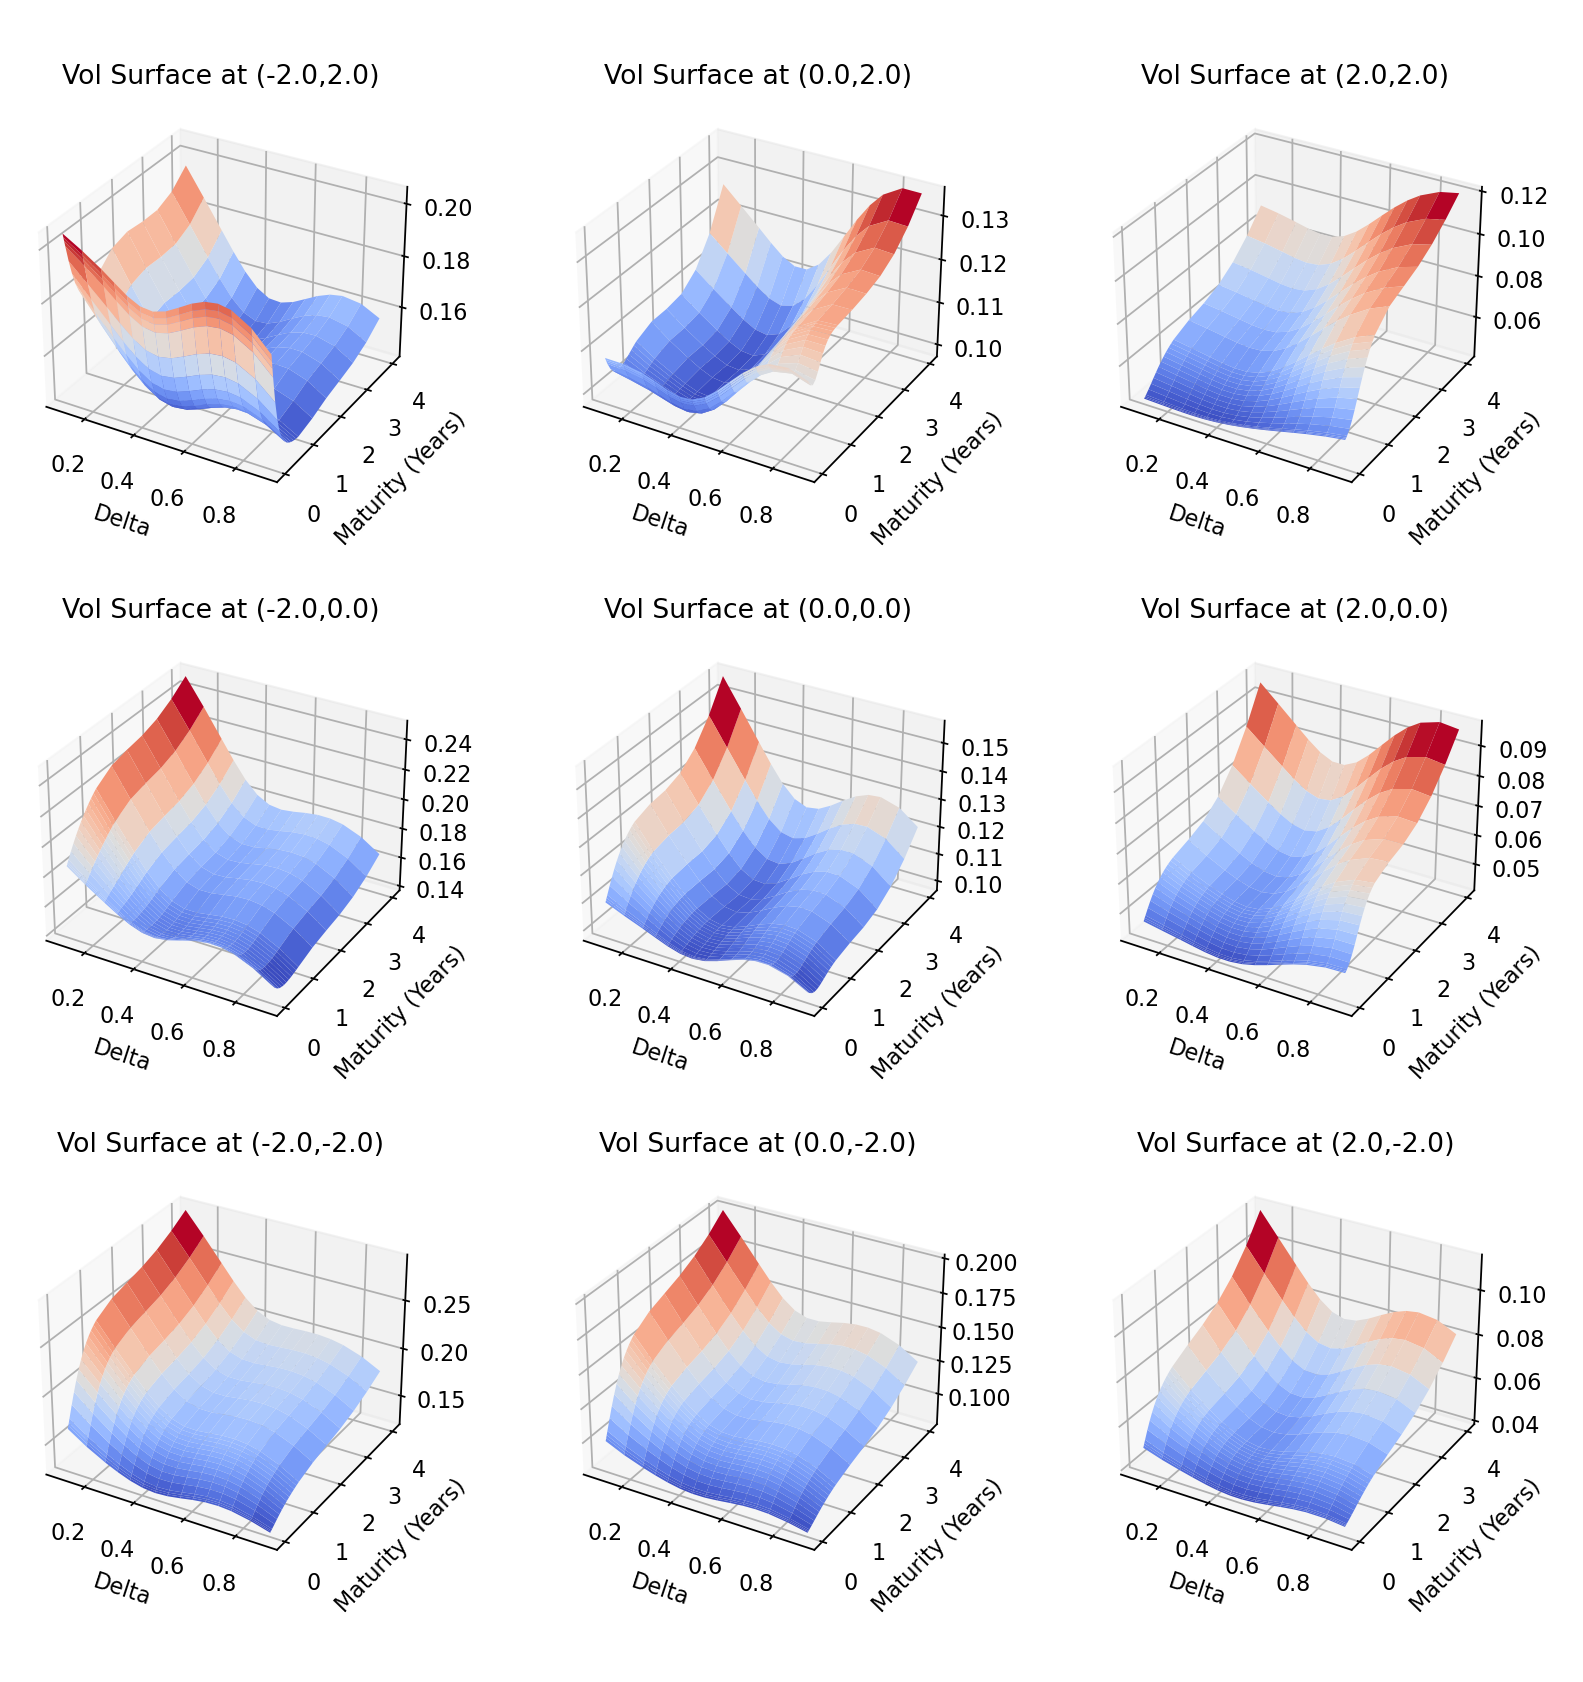
\includegraphics[width=0.8\textwidth,center]{interpolation.png}
    \caption{Examples of synthetic volatility surfaces generated when interpolating across two latent dimensions.}
  \label{fig:interpolation}
\end{center}
\end{figure}


We may wish to observe the behavior of volatility surfaces in specific scenarios.  Exhibit \ref{fig:encodings} shows the encoded latent variables for the volatility surfaces in the validation set. While the majority of the points are clustered near the origin, we notice many outliers which correspond to volatility surfaces observed at the beginning of the international pandemic in March 2020. By sampling latent variables in these outlying regions, we can simulate extreme scenarios that may occur.  



% Training on volatility surfaces from fewer currencies results in better reconstructions, but limits the space of surfaces that can be constructed by the model.



% As the dimensionality reduction provides a simplified view of markets, our model can also be used to analyse the dynamics of the IVS across time. Exogenous factors such as changes in monetary policy, as well as major financial events could be compared to the dynamics of the latent encodings, which are much more expressive than reduced metrics such as market indexes. A plot of the latent encodings over time is illustrated in Exhibit \ref{fig:latent_time}, and left as an amusing exercise for  the intrepid reader to interpret. 


% To further explore the latent encodings, we can interpolate across latent space, visualizing the reconstructed surfaces to identify the learned features. Exhibit \ref{fig:interpolation} depicts surfaces reconstructed by interpolating across both latent dimensions. The characterization of skew and short term volatility appear to be captured by the latent encodings, albeit in a correlated manner. Although VAEs are powerful for capturing non-linear latent features, it is a challenging task to ensure that each of these high-level features is expressed independently by a latent dimension. At this point, it may be tempting to consider PCA as a contender in this regard, producing uncorrelated principal components. In fact, \citet{pca} is one of many works that use PCA to analyze implied volatilities. However, PCA limits our analysis to linear transformations at the cost of expressivity and, more importantly, is unable to generate synthetic surfaces that respect arbitrage conditions.

% To verify that the VAE is indeed producing realistic surfaces, we evaluate it's to ability to calibrate and reconstruct surfaces. Exhibit \ref{fig:smiles} illustrates an example of interpolation for an out-of-sample volatility surface. The model can provide good fits for smiles with more than one inflexion point. Of course, a model could be trained on data for a single currency and provide an even better fit, however, one of the powerful aspects of our approach is that our network was trained using volatility surfaces from \textit{all} currencies in our dataset, showing that our model can generalize well without sacrificing accuracy. 

% To identify areas where the model could be improved, we evaluate the mean absolute error from the mid price to the reconstructed price, as shown in Exhibit \ref{fig:mae_table}. As options with low maturities have the most erratic prices, it is no surprise that this region is the hardest to predict. Note that this model was trained using the mean squared error. In an industrial setting, one could weigh options close to expiry more heavily to account for this. 

% To verify that our model is not overfitting, we examine a surface with high error (see Exhibit \ref{fig:bad_interpolation}). We find that the implied volatilities greatly exceed the range of values seen in the original training set (especially for low time to expiries) and can conclude that our model performs the best when interpolating in latent space rather than extrapolating. 
% To account for this in an industrial setting, we recommend retraining the model periodically with new volatility surfaces as parameters move out of bounds. This is a quick process that can be done within minutes. To determine when the model needs to be retrained, the sensitivities of the implied volatilities with respect to the latent encodings can be used as they are easily obtained through backpropagation.

% \begin{figure}
%     \centering
%     \includegraphics[width=\textwidth]{bad_interpolation.png}
%     \caption{An example where the model performs poorly at interpolation. Error bars show the 5th and 95th percentile of all mid prices in the training set, highlighting how far out-of-sample the data point is.}
%     \label{fig:bad_interpolation}
% \end{figure}

    
% Finally, to evaluate the model's ability to infer missing points on partially observed volatility surfaces. In practice, the IVS is often incomplete, and we simulate this by randomly sampling points from the IVS and using the model to predict the remainder of the surface. For the following experiment, we use a pointwise decoder so that arbitrary grid points can be used. Furthermore, since the surface is only partially observed, we use an external optimizer instead of the encoder to calibrate the model. Exhibit \ref{fig:missing_point_test} shows the mean absolute error across the entire surface for the validation dataset. 
\begin{figure}[h]
  \centering
  \adjincludegraphics[trim={.0\width .0\width .0\width .2\width},width=\textwidth]{latent.png}
  \caption{Latent (colour coded) encodings of implied volatility surfaces}
  \label{fig:encodings}
\end{figure}


\section{Conclusion}
Our results demonstrate that VAEs provide a useful approach to analyzing volatility surfaces empirically. We have described how a VAE can be trained, and used the context of foreign exchange markets as a realistic testing ground. Our results show that volatility surfaces can be captured using VAEs with as few as two latent dimensions and that the resulting models can be used for practical and exploratory purposes. For the sake of concreteness, we limited the scope of this paper to VAEs with Gaussian priors. In future work it should be determined if a VAE model without Gaussian priors is able to learn an even wider range of market behaviours while retaining the stability of our model.


\newpage

\printbibliography
\newpage
\appendix
\begin{appendices}
\section{Arbitrage Conditions}\label{app:arb}
Following \citet{ssvi}, we can specify static arbitrage conditions as follows:
Let $F_t$ denote the forward price at time $t$ and $X=\log{\frac{K}{F_t}}$. Define $w(X, t)=t\cdot\sigma^2(X,t)$ as the total implied variance surface. An IVS is free of \textit{calendar arbitrage} if 
\begin{align}\label{eq:calendar_arb}
  \frac{\partial w}{\partial t} & \geq 0.
\end{align}
Let $w'=\frac{\partial w}{\partial X}$ and $w''=\frac{\partial^2 w}{\partial X^2}$. Suppressing the arguments for $w(X,t)$,  the volatility surface is free of \textit{butterfly arbitrage} if 
\begin{align}
  \label{eq:butterfly_arb}
  g(X, t) := \Big(1-\frac{X w'}{2w}\Big)^2 -
  \frac{w'}{4} \Big(\frac{1}{w}
  + \frac{1}{4}\Big) + \frac{w''}{2} \geq 0.
\end{align}
A volatility surface is said to be free of static arbitrage if the conditions in equation (\ref{eq:butterfly_arb}) and (\ref{eq:calendar_arb}) are met.

If we let  
\begin{align}
\label{eq:cal_loss}
  L_{cal} = \norm{\max\Big(0, -\frac{\partial w}{\partial t}\Big)}^2,
\end{align}
and 
\begin{align}
\label{eq:butt_loss}
  L_{but} = \norm{\max(0, -g)}^2,
\end{align}
the loss function in equation (\ref{eqn:obj}) can then be extended as follows:
\begin{align}
\label{eq:arb_loss}
  \rm{RE} + \beta\rm{KL} + \lambda_{cal} L_{cal} + \lambda_{but} L_{but}.
\end{align}
As the parameters $\lambda_{cal}$ and $\lambda_{but}$ are increased, the possibility of
static arbitrage is reduced. 
\pagebreak

% \begin{figure}[H]
% \centering
%     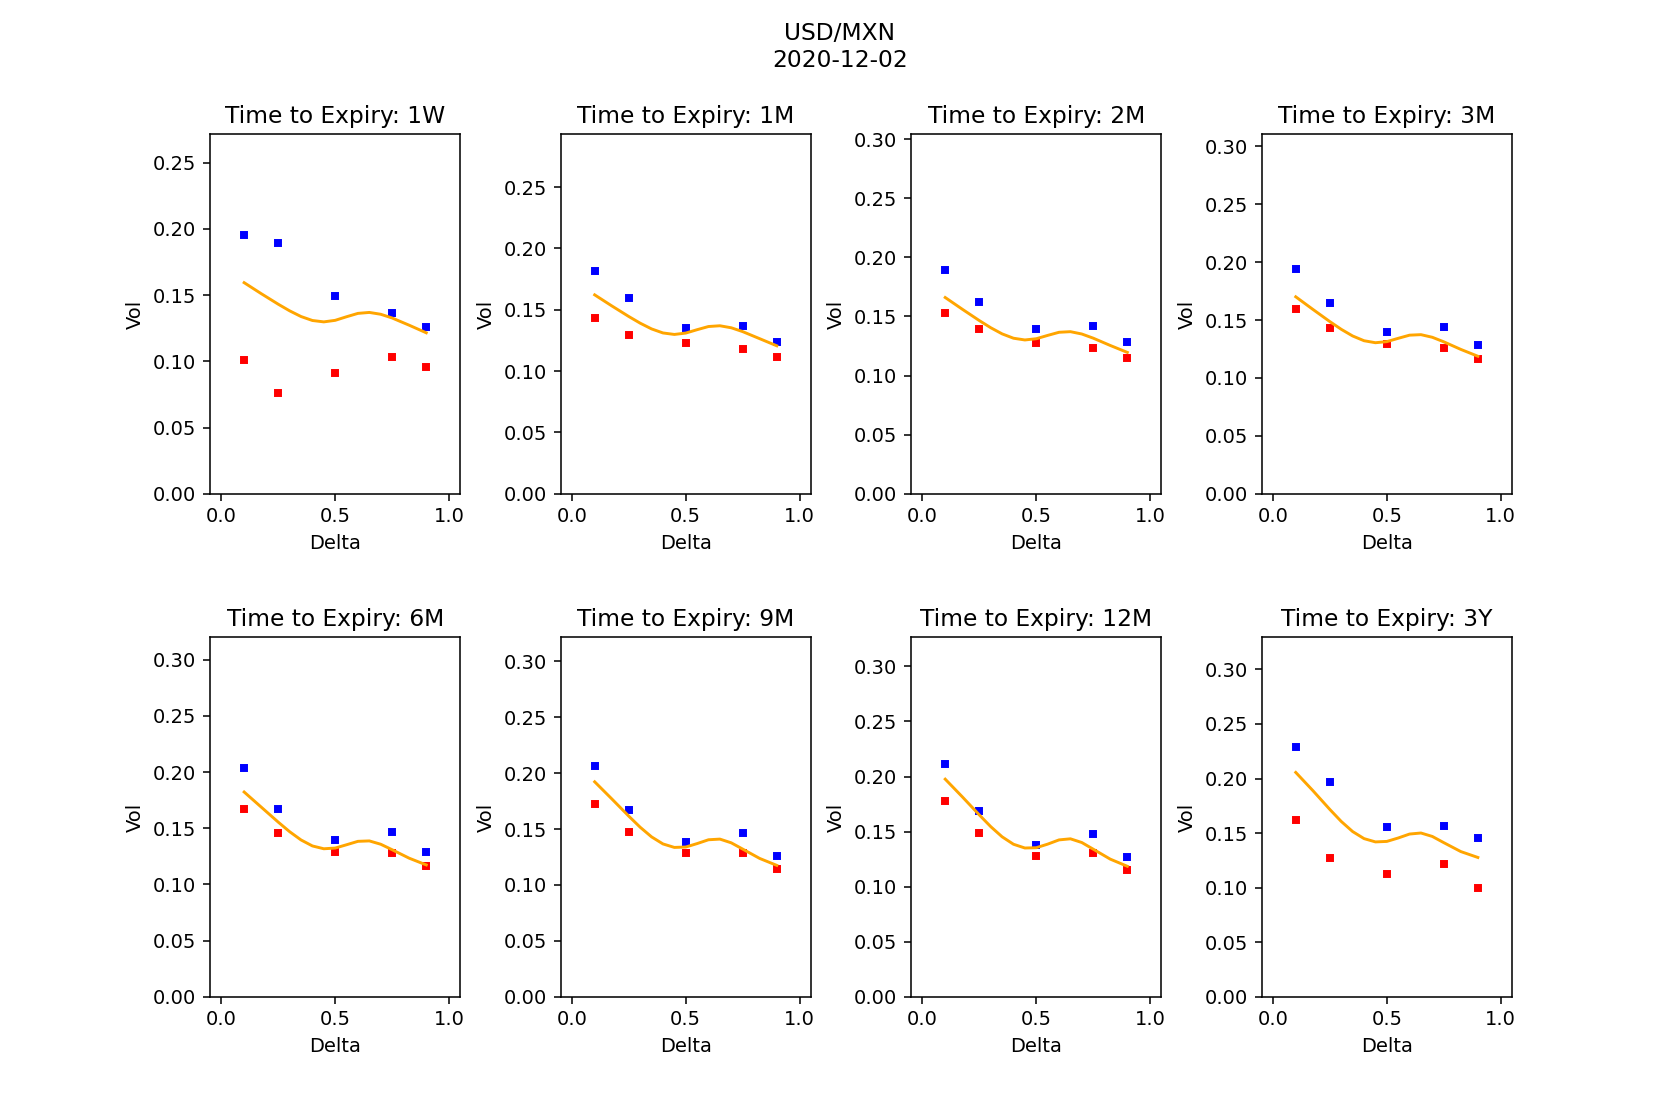
\includegraphics[width=0.8\textwidth]{smile_examples.png}
%   \caption{An example of interpolation results under normal market conditions. The red and blue points represent the bid and ask quotes respectively, while the orange line represents the predicted volatility.}
%     \label{fig:smiles}
% \end{figure}
% \begin{figure}[H]
% \centering
%   \begin{subfigure}{0.4\textwidth}
%   \centering
%     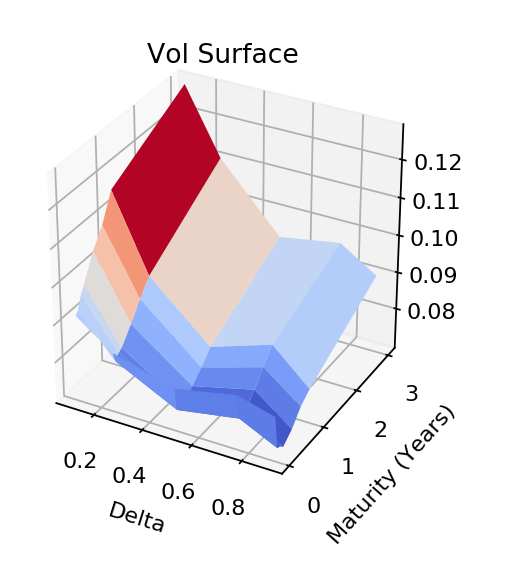
\includegraphics[width=\textwidth]{sample1.png}
%   \caption{Original surface}
%   \end{subfigure}
%   \begin{subfigure}{0.4\textwidth}
%   \centering
%     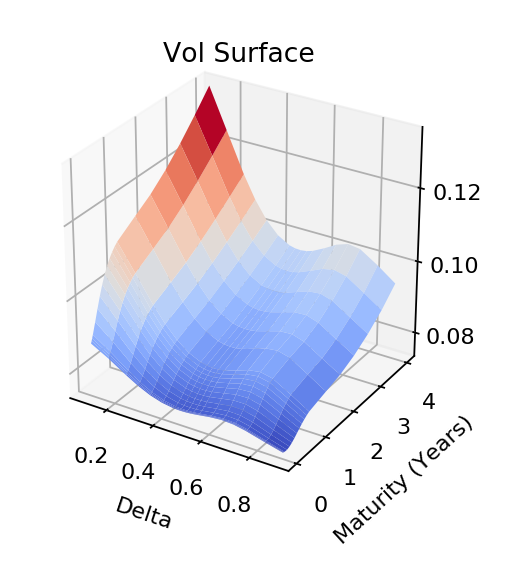
\includegraphics[width=\textwidth]{sample1_reconstruct.png}
%   \caption{Reconstructed surface}
%   \end{subfigure}
%   \caption{An example of a reconstructed, interpolated volatility surface using a VAE trained on foreign exchange data.}
%     \label{fig:example_reconstruction}
% \end{figure}
% \begin{figure}
%     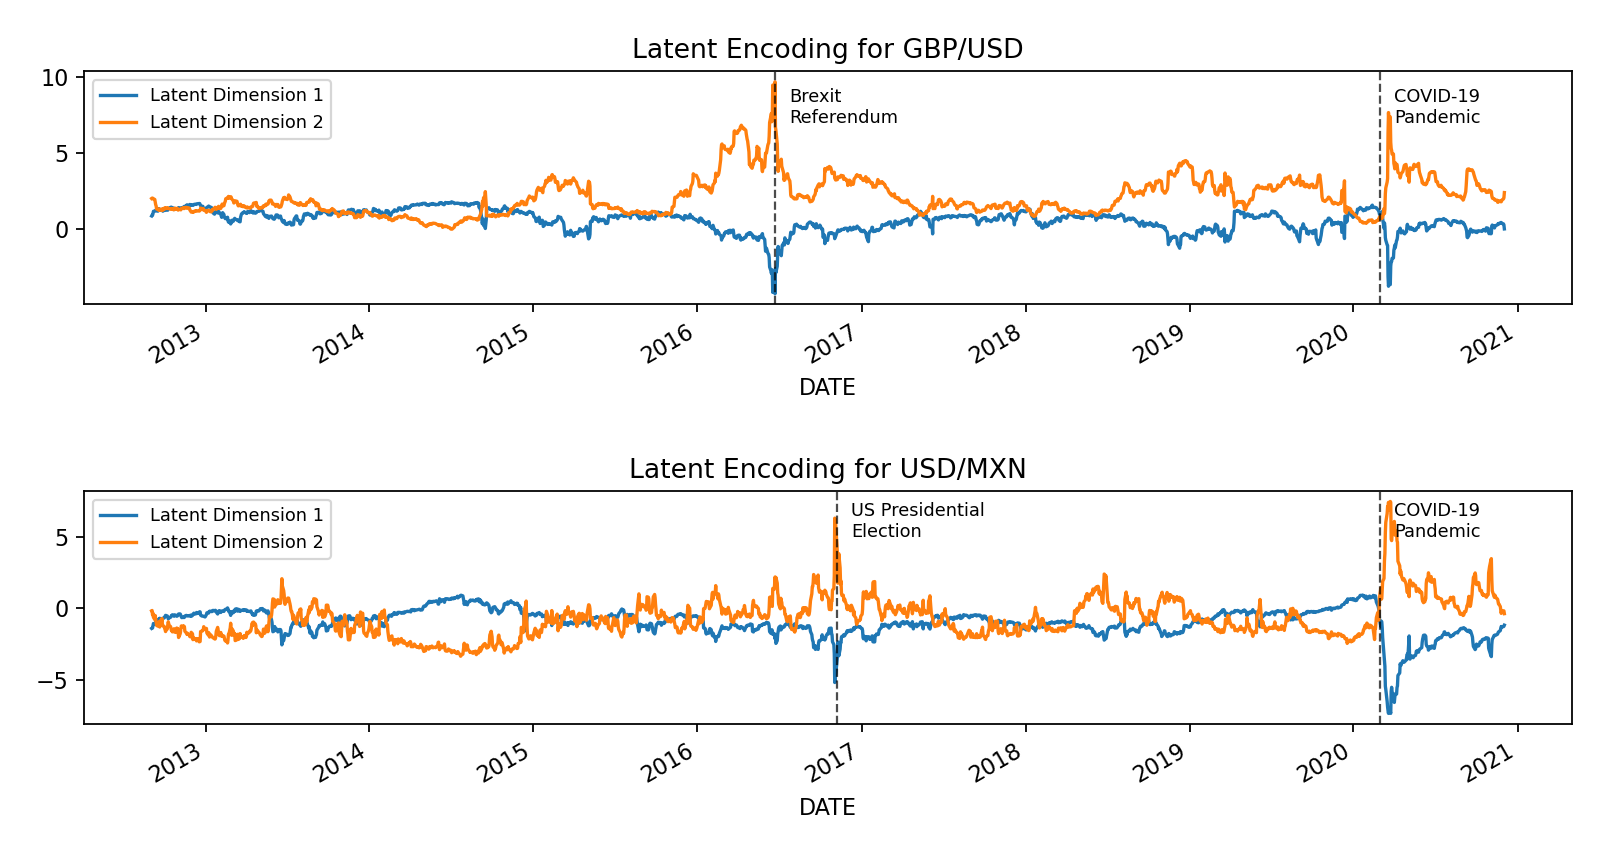
\includegraphics[width=\textwidth]{latent_time.png}
%     \caption{A plot of latent variables against time. We draw attention to the GBP/USD during mid-2016, during the UK's referendum to leave the European Union, as well as the USD/MXN during late-2016, following the results of the US presidential election.}
%   \label{fig:latent_time}
% \end{figure}
% \begin{figure}[hp!]
%     \centering
%     \adjincludegraphics[trim={.05\width .05\width .05\width .05\width},width=1\textwidth]{interpolation_smiles.png}
%     \caption{The one year volatility smiles from the synthetic surfaces in Exhibit \ref{fig:interpolation}. The surfaces are generated by interpolating across two latent dimensions.}
% \end{figure}
% \begin{figure}
%     \centering
%     \adjincludegraphics[trim={.05\width .05\width .05\width .05\width},width=\textwidth]{interpolation_term_structure.png}
%     \caption{The at-the-money term structures from the synthetic surfaces in Exhibit \ref{fig:interpolation}. The surfaces are generated by interpolating across two latent dimensions.}
% \end{figure}
\end{appendices}
\end{document}